\documentclass[14pt,fleqn]{extarticle}
\usepackage[T2A,T1]{fontenc}
\usepackage[utf8]{inputenc}
\usepackage[russian]{babel}
\usepackage{amsmath}
\usepackage{graphicx}
\usepackage{tabularx}
\usepackage{boldline}
\usepackage{makecell}
\usepackage{arydshln}
\usepackage{mathtools}
\usepackage{centernot}
\usepackage{enumitem}
\usepackage{nccmath}
\usepackage[a4paper, total={6.5in, 9.5in}]{geometry}

\graphicspath{ {./images/} }
\setlength{\mathindent}{0pt}
\setlength\parindent{0pt}

\def\at{
	\left.
	\vphantom{\int}
	\right|
}


\begin{document}
	\begin{titlepage}
		
\includegraphics[scale=0.12]{logo}
		\begin{center}
			\textbf{МИНОБРНАУКИ РОССИИ}\\
			\vspace{0.2cm}
			\textbf{Федеральное государственное бюджетное образовательное учреждение высшего образования}\\
			\textbf{<<САНКТ-ПЕТЕРБУРГСКИЙ ГОСУДАРСТВЕННЫЙ ЭКОНОМИЧЕСКИЙ УНИВЕРСИТЕТ>>}\\
			\vspace{0.6cm}
			Факультет информатики и прикладной математики\\
			Кафедра прикладной математики и экономико-математических методов\\
			\vspace{1cm}
			\textbf{ОТЧЁТ}\\
			по дисциплине:\\
			\textbf{<<Имитационное моделирование>>}\\
			на тему:\\
			\textbf{<<Построение пешеходной модели. Станция метро Озерки>>}\\
		\end{center}
		\vspace{1cm}
		Направление: 01.03.02\\
		Обучающийся: Бронников Егор Игоревич\\
		Группа: ПМ-1901\\
		\vfill
		\begin{center}
			Санкт-Петербург\\
			2022\\
		\end{center}
	\end{titlepage}
	\subsection*{Задание}
	Построить и проанализировать пешеходную имитационную модель станции метро Озерки.

	\subsection*{Описание модели}
	Имеется следующая схема станции метро Озерки. (Рисунок \ref{fig:metro_plan})
	\begin{figure}[h]
		\centering 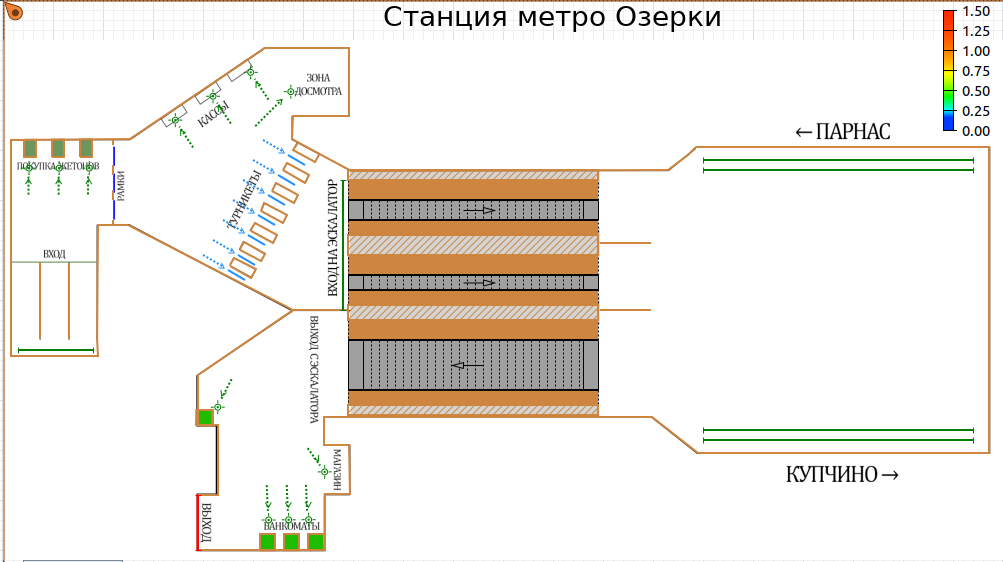
\includegraphics[scale=0.5]{metro_plan}
		\caption{Схема станции метро Озерки}
		\label{fig:metro_plan}
	\end{figure}
	
	При входе пассажиры могут купить жетоны либо в специальных автоматах, либо пойти на кассу, также их могут остановить на досмотр. После чего пассажиры проходят через турникеты и спускаются по эскалатору, далее они выбирают направление движения и садятся на поезд.\\
	
	Соответственно, пассажиры, которые прибывают на станцию метро с других направлений, могут пройти по эскалатору на верх. После того как они поднялись, у них есть выбор пойти в группу банкоматов, пойти в <<непопулярный>> банкомат или зайти в магазин, также в магазине они смотрят на товар и в случае, если там нет нужного им продукта покинуть магазин или купить что-то. После всех данных альтернатив пассажиры покидают станцию метро.
	
	\newpage
	
	\subsection*{Реализация модели}
	
	В соответствии с описанием данная модель была реализована в среде моделирования \textit{AnyLogic} (Рисунок \ref{fig:metro_anylogic_model}).
	
	\begin{figure}[h]
		\centering 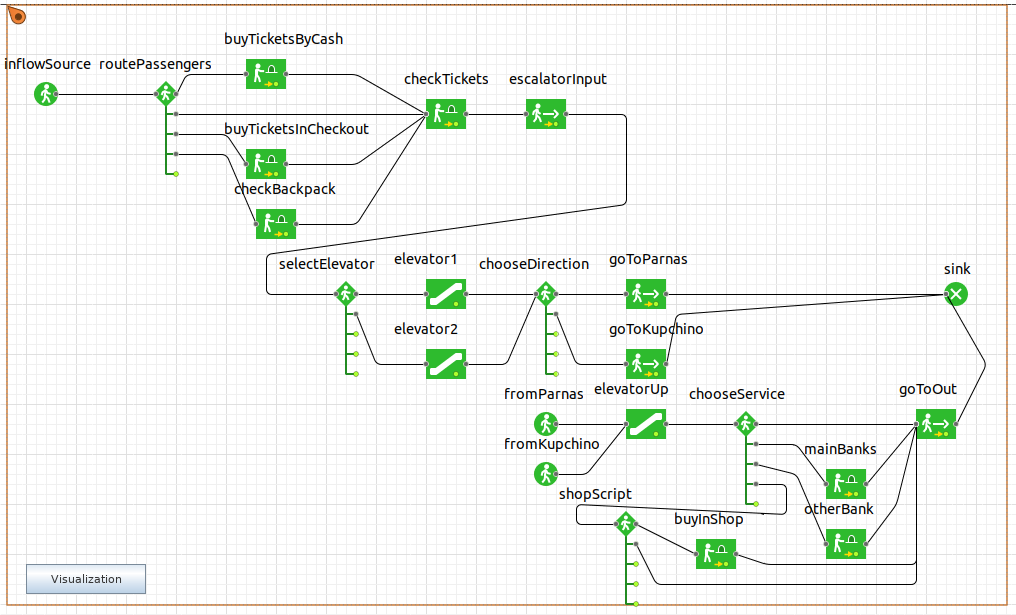
\includegraphics[scale=0.3]{metro_anylogic_model}
		\caption{Модель в среде \textit{AnyLogic}}
		\label{fig:metro_anylogic_model}
	\end{figure}

	Данная модель не имеет модификаций с изменением направления эскалатора и имеет статический потом интенсивности пассажиров.\\
	
	Также в соседнем окне была построена визуализация модели и тепловая карта, которая соответствует плотности различных участков станции. (Рисунок \ref{fig:metro_visualization})
	
	\begin{figure}[h]
		\centering 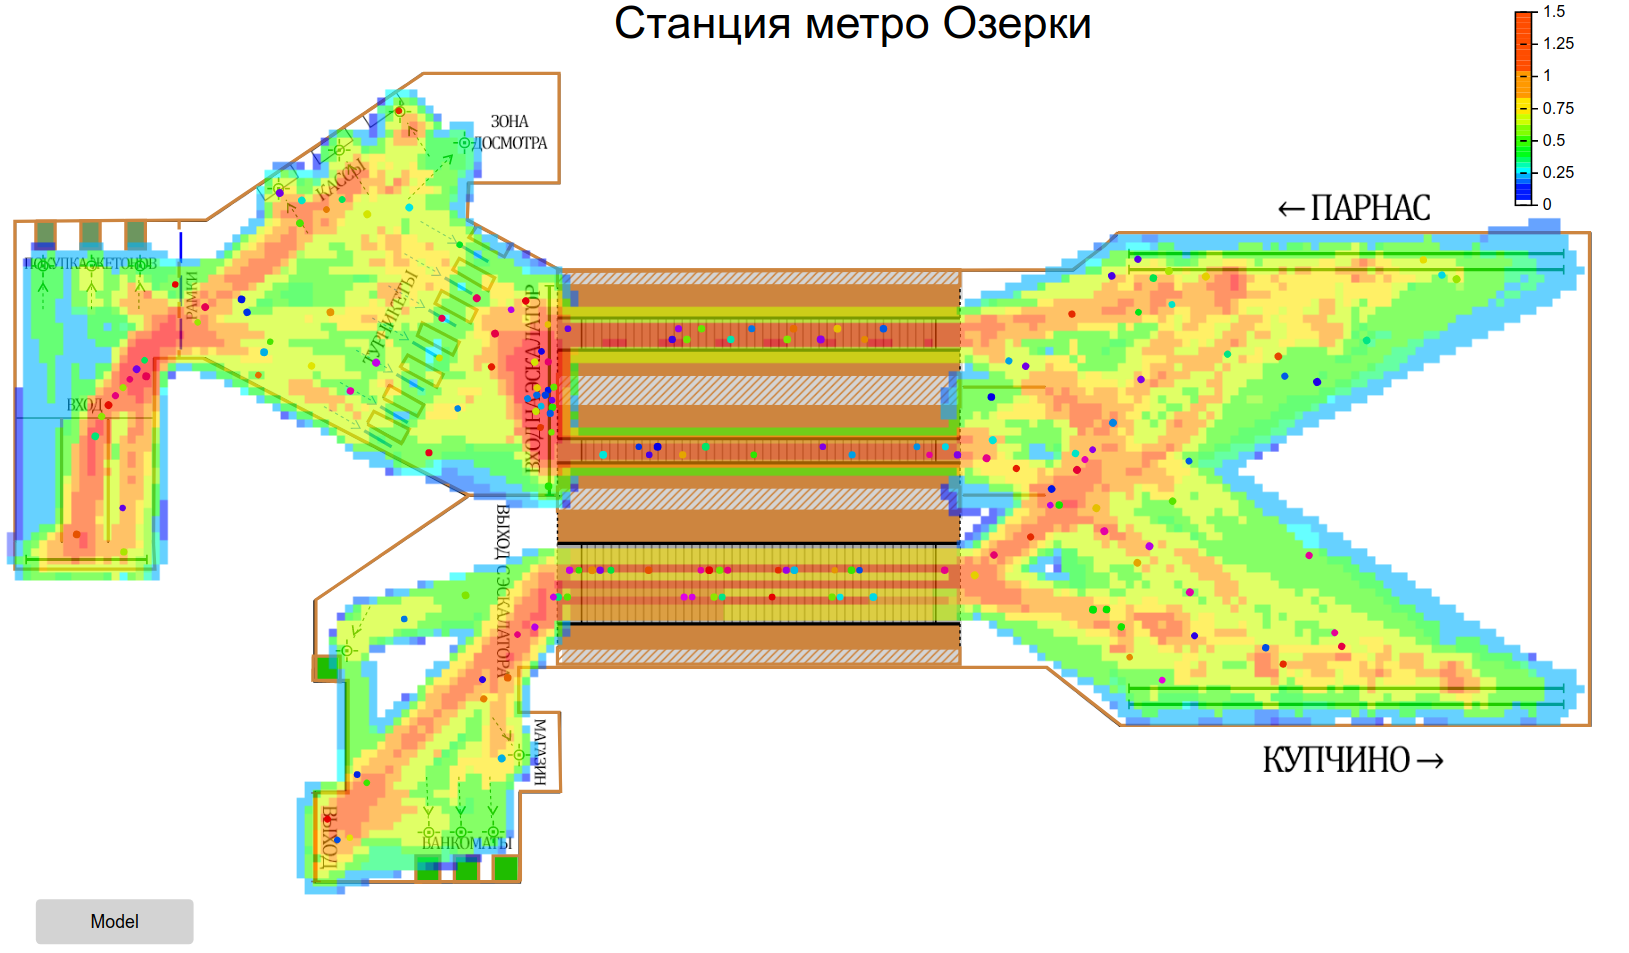
\includegraphics[scale=0.24]{metro_visualization}
		\caption{Модель в среде \textit{AnyLogic}}
		\label{fig:metro_visualization}
	\end{figure}

	\newpage
	
	На данной тепловой карте можно видеть, что если средняя интенсивность пассажиропотока составляет 2000 человек в час, то <<узким горлышком>> на станции служит вход до рамок металлодетектора и входа на спуск по эскалатору.
\end{document}
